%%%%%%%%%%%%%%%%%%%%%%% CHAPTER - 4 %%%%%%%%%%%%%%%%%%%%\\
\chapter{Methodology}
\label{C4} %%%%%%%%%%%%%%%%%%%%%%%%%%%%
\graphicspath{{Figures/Chapter-4figs/PDF/}{Figures/Chapter-4figs/}}
% \noindent\rule{\linewidth}{2pt}
%%%%%%%%%%%%%%%%%%%%%%%%%%%%%%%%%%%%%%%%%%%%%%%%%%%%%%%%%%%%%%%%%%%%%%%%%%%%%%%%%%
\section{Proposed System} \label{S4.1}
The proposed AI-Powered Cricket Batting Analysis System follows a structured methodology that integrates deep learning, computer vision, and a client–server mobile architecture to achieve real-time shot classification and feedback.

The methodology begins with dataset collection and preparation, where over 8000 cricket batting images were gathered and categorized into predefined shot classes along with an unknown class. The images were preprocessed through resizing, normalization, and data augmentation techniques to improve model performance and generalization. The dataset was then divided into training and testing sets for model development.

Next, a YOLOv8 deep learning model was trained using the Ultralytics framework in Google Colab. The model learned important visual features such as player posture, bat orientation, and body alignment to detect and classify different cricket batting shots. After achieving satisfactory performance, the trained model was exported and integrated into the backend server for real-time inference.

In the deployment phase, the trained model was integrated into a Python Flask-based backend server developed in VS Code. The server is responsible for receiving images from the Android application, preprocessing them, performing model inference, and generating a prediction result. The server then converts the processed output image into Base64 format and sends it back to the client in JSON format.

On the client side, an Android application developed using Android Studio captures the player’s image through CameraX and sends it to the backend server using Retrofit. Upon receiving the server response, the application displays the predicted shot category along with the processed image and provides voice feedback using Text-to-Speech.

Thus, the proposed system methodology ensures efficient data flow from image capture to prediction and feedback, enabling real-time, automated cricket shot analysis through a reliable and scalable client–server architecture.
\begin{figure}
	\centering
	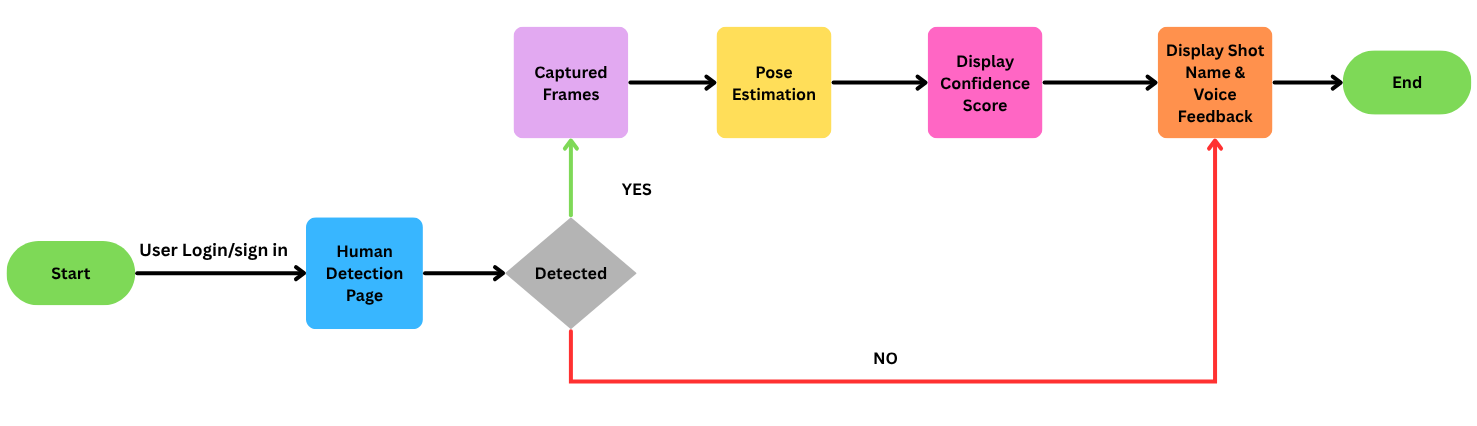
\includegraphics[width=1.05\linewidth]{Figures/Chapter-4figs/block_diagram}
	\caption{Block Diagram}
	\label{fig:blockdiagram}
\end{figure}

\section{Android App} \label{S4.2}
The AI-Powered Cricket Batting Analysis system is implemented as an Android application to improve accessibility and practical usability. The mobile application enables players to capture their batting images directly using their smartphone camera during practice sessions. The captured image is transmitted to the backend server, where the trained deep learning model performs shot classification and analysis.

The Android app interface provides:
\begin{itemize}
	\item Camera Capture Option, allowing users to capture batting images in real-time using CameraX integration.
	\item Server Connectivity Module, enabling image upload to the Flask backend server via Retrofit API.
	\item Live Prediction Display, showing the classified shot category along with the processed output image returned from the server.
	\item Instant Voice Feedback, using Text-to-Speech functionality to announce the predicted result.
	\item Server Configuration Option, allowing dynamic IP address entry for flexible client–server communication.
	\item Error Handling and Status Indicators, ensuring smooth user interaction during image upload and result retrieval.
\end{itemize}
	
This application allows players to practice anywhere using only a smartphone and internet connection, eliminating the need for expensive motion-tracking equipment and making AI-based cricket training portable, affordable, and efficient.

\section{Image Data Collection} \label{S$.3}
The data collection stage forms the foundation of the model development process. The system requires multiple image samples of each batting shot captured under consistent and controlled conditions to ensure accurate classification performance.
\begin{itemize}
	\item Camera Placement: Smartphone camera positioned approximately 3–4 meters from the batsman at waist or shoulder height for clear full-body visibility.
	\item Image Resolution: Minimum 224×224 pixels after preprocessing to match model input size.
	\item Lighting Conditions: Uniform lighting to reduce shadows and improve feature extraction accuracy.
	\item Background: Simple or less cluttered background to clearly isolate the batsman’s posture and bat position.
	\item Camera Angle: Side or slightly angled view to clearly capture body posture and bat swing direction.
\end{itemize}

The dataset consists of 8000+ labeled images representing four different batting shot categories along with an additional unknown class to improve generalization. Each shot type was captured multiple times with variations in posture, angle, and player style to enhance diversity.\\
The collected dataset was divided into:
\begin{itemize}
	\item Training Set – 70\% (for model learning)
	\item Testing Set – 20\% (for performance evaluation)
	\item Validation Set – 10\% (for tuning and accuracy improvement)
\end{itemize}
This structured data collection approach ensures better model training, improved accuracy, and robust real-world performance.
%%%%%%%%%%%%%%%%%%%%%%%%%%%%%%%%%%%%%%%%%%%%%%%% Section-1 %%%%%%%%%%%%%%%%%%%%%%%%%%%%%%%%%%%%%%%%%%%%%%%%%%%%%%%%%%%%%%%%%%%%%%%%%%%%


%%%%%%%%%%%%%%%%%%%%%%%%%%%%%%%%%%%%%%%%% Figure 4.1 %%%%%%%%%%%%%%%%%%%%%%%%%%%%%%%%%%%%%%%%%%%%%%%%%%%%%%%%%%%%%%%%%%%%%%%%%%%%%%%
%%%%%%%%%%%%%%%%%%%%%%%%%%%%%%%%%%%%%%%%%%%%%%%%%%%% Section-2 
\section{Data Preprocessing} \label{S4.4}
Before model training, the collected image dataset undergoes several preprocessing steps to ensure consistency, improve model performance, and enhance generalization capability:

\begin{itemize}
	\item Image Resizing: All images are resized to a fixed dimension (e.g., 224×224 pixels) to match the input size required by the YOLOv8 model and maintain uniformity.
    \item Normalization: Pixel values are scaled to a range of 0–1 to improve numerical stability and accelerate the learning process during training.
    \item Data Cleaning: Blurred, low-quality, or irrelevant images are removed to maintain dataset quality and prevent inaccurate predictions.
    \item Background Handling: Minor noise reduction techniques are applied where necessary to reduce background distractions and focus on the player’s posture and bat position.
    \item Data Augmentation: Techniques such as rotation, horizontal flipping, zooming, and brightness adjustment are applied to increase dataset diversity and reduce overfitting.
    \item Label Encoding: Each image is assigned a categorical label corresponding to its shot class, including an additional unknown class to improve robustness.
\end{itemize}
These preprocessing steps ensure that the model learns important visual features such as body posture, bat angle, and stance alignment accurately, regardless of lighting conditions or background variations.

\section{Shot Classification Process} \label{S4.5}
The shot classification process identifies the type of batting shot from the captured image using a trained You Only Look Once(YOLOv8) model. Instead of extracting skeletal keypoints, the system analyzes visual posture patterns directly from the image to determine the correct category.

Using a trained deep learning model built with TensorFlow/Keras, the system processes the input image and extracts important spatial features such as body alignment, bat angle, arm extension, leg positioning, and overall stance balance. These features are learned automatically during training using the 8000+ labeled dataset.

Each input image is represented as a matrix of pixel values (after resizing and normalization). The YOLOv8 model processes the image through multiple deep learning layers to extract meaningful visual patterns that help identify different cricket batting shots.

The architecture performs the following operations:
\begin{itemize}
	\item Feature Extraction: The YOLOv8 backbone network extracts important visual features such as player posture, bat direction, and body alignment.
	\item Feature Aggregation: The neck layer combines features from different scales to improve detection of relevant patterns in the image.
	\item Object Detection and Classification: The detection head predicts the location of the player and classifies the batting shot into the predefined categories.
	\item Confidence Prediction: The model outputs confidence scores for each predicted class, including the unknown category, indicating the likelihood of the detected shot.
\end{itemize}
The system selects the class with the highest probability score as the final prediction. If the prediction confidence is low, the image is classified as unknown to avoid misclassification.

This process enables accurate and efficient shot identification based purely on visual posture analysis, making the system practical for real-time AI-based cricket training.

\section{Shot Estimation Process} \label{S4.6}
After image preprocessing and feature extraction, the system identifies which batting shot the player attempted based on learned visual posture patterns. Instead of joint angle calculations, the classification is performed using a trained You Only Look Once(YOLOv8) model that recognizes distinctive body alignment, bat position, and stance characteristics.

Each shot category in the dataset is characterized by unique visual features such as bat swing direction, body posture, leg positioning, and weight distribution. These visual cues enable the model to accurately differentiate between shot types.
\begin{table}[h]
	\centering
	\caption{Batting Shot Categories}
	\renewcommand{\arraystretch}{1.4}
	\begin{tabular}{|p{4cm}|p{10cm}|}
		\hline
		\textbf{Shot Category} & \textbf{Distinct Visual Features} \\
		\hline
		
		Straight Drive &
		Characterized by a vertical bat swing with strong forward body alignment and balanced weight transfer to the front foot. \\
		\hline
		
		Pull Shot &
		Identified by horizontal bat movement with upper-body rotation and weight shift toward the back leg. \\
		\hline
		
		Cut Shot &
		Recognized by angled bat direction with lateral body movement and open shoulder alignment. \\
		\hline
		
		Sweep Shot &
		Shows lowered body posture with bent knees and bat swung close to the ground in a sweeping motion. \\
		\hline
		
		Unknown Class &
		Used when posture does not match any trained shot patterns or prediction confidence is below threshold. \\
		\hline
		
	\end{tabular}
\end{table}

The system uses a trained deep learning classifier built with TensorFlow/Keras to analyze extracted image features and categorize the input into the correct shot class. The Softmax output layer generates probability scores for each shot, and the class with the highest probability is selected as the final prediction.

This approach ensures accurate and efficient identification of straight drive, pull shot, cut shot, and sweep shot using image-based visual pattern recognition, making the system suitable for real-time AI-powered cricket training applications.
\begin{itemize}
	\item Automated shot classification using Artificial Intelligence and deep learning for accurate and reliable feedback.
	\item Real-time prediction and instant result display during batting practice sessions.
	\item Cost-effective virtual coaching system that eliminates the need for expensive motion-tracking equipment or professional trainers.
	\item Simple and user-friendly Android mobile interface for easy image capture and result viewing.
	\item Portable and accessible solution that allows players to practice anytime and anywhere.
	\item Client–server architecture that efficiently handles heavy processing on the backend server.
	\item Scalable system design that allows addition of new shot categories and advanced features in the future.
	\item Unknown shot detection mechanism to minimize misclassification and improve prediction reliability.
	\item Enhances overall training efficiency by providing consistent and quick performance evaluation.
\end{itemize}

\section{Performance Evaluation} \label{S4.7}
The performance evaluation process measures how accurately the system classifies the player’s batting shot based on the trained deep learning model. Instead of joint-angle deviation, the evaluation is performed using classification metrics derived from model predictions.

For each test image, the model calculates a probability score (0–1) for each shot category using the Softmax output layer:
\[
P(class_i) = \frac{e^{z_i}}{\sum_{j=1}^{n} e^{z_j}}
\]
Where:
\begin{itemize}
	\item $(z_i)$ represents the output score of class $i$ before activation.
	\item $(n)$ represents the total number of shot classes including the unknown class.
\end{itemize}
The class with the highest probability score is selected as the final prediction.

To evaluate overall model performance, the following metrics are used:
\begin{itemize}
	\item Accuracy – Percentage of correctly classified images out of total test images.
	\item Precision – Measures how many predicted shots were actually correct.
	\item Recall – Measures how well the model identifies all actual instances of each shot.
	\item F1-Score – Harmonic mean of precision and recall for balanced evaluation.
	\item Confusion Matrix – Displays correct and incorrect predictions across all shot categories.
\end{itemize}

\section{Feedback Mechanism} \label{S4.8}
	
The feedback module acts as the intelligent coach interface of the AI-Powered Cricket Batting Analysis System. After the captured image is processed and the shot is classified by the deep learning model, the system delivers instant feedback to help the player understand their performance.
\begin{itemize}
    \item Visual Display: Shows the predicted shot name clearly on the screen along with the processed image returned from the server. This allows the player to immediately verify the recognized shot.
	\item Confidence Indicator: Displays the prediction confidence score (if enabled), helping users understand the reliability of the classification result.
	\item Text-Based Feedback: Provides short on-screen messages such as “Correct Shot Detected” or “Unrecognized Shot – Try Again” when the prediction confidence is low.
	\item Audio Guidance: Uses Text-to-Speech (TTS) functionality to announce the predicted shot category, enabling hands-free feedback during practice sessions.
    \item Unknown Shot Alert: If the image does not match trained categories or falls below the confidence threshold, the system labels it as “Unknown,” preventing incorrect evaluation.
\end{itemize}
This feedback mechanism enables players to practice independently while receiving immediate AI-based guidance, thereby improving consistency, accuracy, and overall batting performance over time.

\section{Model Architecture and Training Strategy} \label{S4.9}
The core of the proposed system is a YOLOv8 (You Only Look Once version 8) model designed for multi-class image classification. The model was trained using a dataset of 8000+ labeled images representing four batting shots along with an unknown class.

The YOLOv8 architecture performs real-time object detection and classification by processing the entire image in a single forward pass. It utilizes advanced feature extraction layers along with optimized detection heads to identify and classify batting poses efficiently. The model learns important visual patterns such as bat angle, body alignment, shoulder rotation, and leg positioning, enabling accurate and fast prediction.

After feature extraction, the output is flattened and passed through Fully Connected (Dense) layers for classification. The final layer uses a Softmax activation function to generate probability scores for each shot category. The model was compiled using:
\begin{itemize}
	\item Loss Function: Categorical Crossentropy (for multi-class classification)
    \item Optimizer: Adam optimizer
    \item Evaluation Metric: Accuracy
\end{itemize}
To improve generalization and prevent overfitting, techniques such as data augmentation, validation splitting, and proper epoch tuning were applied. The model was trained and tested using Google Colab with GPU acceleration, ensuring efficient training performance.

\section{Client–Server Communication and API Integration} \label{S4.10}
The system follows a structured client–server architecture, where the Android application acts as the client and the Flask-based backend server performs model inference.

When the user captures an image through the Android application, the image is temporarily stored and sent to the backend server using a multipart HTTP POST request via the Retrofit networking library. The server receives the image through a defined Flask API endpoint.

On the server side, the image undergoes preprocessing (resizing and normalization) before being passed into the trained YOLOv8 model for prediction. The model generates a probability distribution across all shot classes, and the highest probability class is selected as the final output.

The server then encodes the processed image into Base64 format and sends a structured JSON response containing:
\begin{itemize}
	\item Predicted shot label
	\item Confidence score
	\item Encoded processed image
\end{itemize}

The Android application receives this response, decodes the image, displays the result on the screen, and provides voice feedback using Text-to-Speech. Proper error handling mechanisms are implemented to manage network failures or invalid inputs.

This structured communication ensures smooth data flow, efficient processing, and real-time feedback delivery between the mobile application and the AI model.
